% WSCG sample document 
%
% based on Gabriel Zachmann's sample
% http://zach.in.tu-clausthal.de/latex/
%
% modified Apr 2012 to match WSCG Word template
%
\documentclass[twoside,twocolumn,10pt]{article}
%\documentclass[twoside,twocolumn,draft]{article}

%  for debugging
%\tracingall%\tracingonline=0
%\tracingparagraphs
%\tracingpages


%%%%%%%%%%%%%%%%%%%%%%%%%%%%%%%%%%%%%%%%%%%%%%%%%%%%%%%%%%%%%%%%%%%%%%%%%%%%%
%                             Packages

\usepackage{wscg}           % includes a number of other packages (e.g., myalgorithm)
\RequirePackage{ifpdf}
\ifpdf
 \RequirePackage[pdftex]{graphicx}
 \RequirePackage[pdftex]{color}
\else
 \RequirePackage[dvips,draft]{graphicx}
 \RequirePackage[dvips]{color}
\fi
%\usepackage[german,english]{babel}     % default = english
%\usepackage{mypicture}      % loads graphicx.sty, color.sty, eepic.sty
%\usepackage{array}          % better tabular's & arrays, plus math tabular's
%\usepackage{tabularx}      % for selfadjusting p-columns
%\setlength{\extrarowheight}{1ex}   % additional space between rows
%\usepackage{booktabs}      % typographically much better
%\usepackage{mdwlist}        % for compacted lists, and more versatile lists
%\usepackage[intlimits]{amsmath} % more math stuff, see texdoc amsldoc
%\usepackage{mymath}         % own commands, loads amssymb & array.sty
%\usepackage{hyphenat}      % hyphenatable -, /, etc.
%\usepackage{theorem}
%\usepackage[sort&compress]{natbib}% better \cite commands, more flexible
%\usepackage[sort&compress,super]{natbib} % better \cite commands, more flexible
%\newcommand{\citenumfont}[1]{\textit{#1}}


\usepackage{nopageno}       % no page numbers at all; uncomment for final version



%%%%%%%%%%%%%%%%%%%%%%%%%%%%%%%%%%%%%%%%%%%%%%%%%%%%%%%%%%%%%%%%%%%%%%%%%%%%%
%                                Title

\title{Intuitive Transfer Function Editing Using Relative Visibility Histograms}

\author{
%\parbox{0.25\textwidth}{\centering
%First Author\\[1mm]
%author's affiliation\\
%1st line of address\\
%2nd line of address\\
%Country (ZIP) code, City, State\\[1mm]
%e@mail
%}
%\hspace{0.05\textwidth}
%\parbox{0.25\textwidth}{\centering
%Second Author\\[1mm]
%author's affiliation\\
%1st line of address\\
%2nd line of address\\
%Country (ZIP) code, City, State\\[1mm]
%e@mail
%}
%\hspace{0.05\textwidth}
%\parbox{0.25\textwidth}{\centering
%Third Author\\[1mm]
%author's affiliation\\
%1st line of address\\
%2nd line of address\\
%Country (ZIP) code, City, State\\[1mm]
%e@mail
%}
}

%%%%%%%%%%%%%%%%%%%%%%%%%%%%%%%%%%%%%%%%%%%%%%%%%%%%%%%%%%%%%%%%%%%%%%%%%%%%%
%                          Hyperref


% no hyperlinks
\usepackage{url}
\urlstyle{tt}

% Donald Arsenau's fix for missing kerning of "//" and ":/"
\makeatletter
\def\Uslash{\mathbin{\mathchar`\/}\@ifnextchar{/}{\kern-.15em}{}}
\g@addto@macro\UrlSpecials{\do \/ {\Uslash}}
\def\Ucolon{\mathbin{\mathchar`:}\@ifnextchar{/}{\kern-.1em}{}}
\g@addto@macro\UrlSpecials{\do : {\Ucolon}}
\makeatother





%%%%%%%%%%%%%%%%%%%%%%%%%%%%%%%%%%%%%%%%%%%%%%%%%%%%%%%%%%%%%%%%%%%%%%%%%%%%%
%                              My Commands


%\DeclareMathOperator{\sgn}{sgn}

%\theorembodyfont{\upshape}
%\theoremstyle{break}
%\theoremheaderfont{\bfseries\normalsize}

%\newtheorem{lem}{Lemma}
%\newtheorem{defn}{Definition}

%%%%%%%%%%%%%%%%%%%%%%%%%%%%%%%%%%%%%%%%%%%%%%%%%%%%%%%%%%%%%%%%%%%%%%%%%%%%%
% packages for this paper
\usepackage{amsmath}
\DeclareMathOperator*{\argmax}{argmax} % thin space, limits underneath in displays

\usepackage{hyperref}
\graphicspath{{figures/}{images/}{pictures/}{./}} % where to search for the images
%\usepackage[T1]{fontenc}
%\usepackage[utf8]{inputenc}
%%%%%%%%%%%%%%%%%%%%%%%%%%%%%%%%%%%%%%%%%%%%%%%%%%%%%%%%%%%%%%%%%%%%%%%%%%%%%
%                                Document


\begin{document}

\twocolumn[{\csname @twocolumnfalse\endcsname

\maketitle  % full width title


\begin{abstract}
\noindent
In this paper, we present an interactive approach for intuitively editing colors and opacity values in transfer functions for volume visualization. We introduce the concept of a relative visibility histogram, which represents the difference between the global visibility distribution across the full volume and the local visibility distribution within a user-selected region in the viewport. From this measure we can infer what the user intends to select when they click on a specific region in the viewport and use this result to directly modify the relevant parts of the transfer function.
In addition to direct editing of the transfer function, we also introduce transfer function components which represent the visually dominant features in the user-selected regions.
The user can manipulate the colors and opacity values of the components and merge them to create new transfer functions.
Our approach is lightweight compared to similar techniques and performs in real-time.

\end{abstract}

\subsection*{Keywords}
%Keywords are your own designated keywords - Times New Roman, 10pts.
Volume rendering, transfer function, visibility, visibility histograms
\vspace*{1.0\baselineskip}
}]



%%%%%%%%%%%%%%%%%%%%%%%%%%%%%%%%%%%%%%%%%%%%%%%%%%%%%%%%%%%%%%%%%%%%%%%%%%%%%


\section{Introduction}

\copyrightspace

%Although users typically have a general idea of which parts of the volume should be emphasized for a given task, adjusting the color and alpha values in the transfer function is by no means intuitive, due to the non-linear relationship between the color and alpha of intensity ranges in the transfer function and the visibility voxels in the final image. In fact, visibility in the final image is dependent on the color and alpha of voxels as well as view-dependent occlusion by other objects.

A recurring challenge in volume visualization, is defining effective transfer functions (TF), which assign color and opacity (alpha value) to specific data ranges for visualization. Due to the non-linear relationship between the transfer function and the resultant rendering, the process of editing transfer functions is often counter-intuitive, typically necessitating a trial-and-error process. This may be addressed using an output sensitive approach where the user can more directly control the appearance of the visualization, without explicit knowledge of the transfer function. 

In this paper we propose a technique which enables us to infer a user's intended changes to the visualization, when they click or select a region in the rendered image of a 3D volume data set. This is done by weighting the data in the selected region based on the proportion of materials visible to the user within that region. We introduce the concept of a \emph{relative visibility histogram}, derived from the relationship between the global visibility and the local visibility of data in the user-selected region.
Based on this weighting, the user can directly modify colors and opacity of the volume data, in a manner analogous to painting a 3D scene.
In addition, we introduce an automated technique for creating transfer function components from relative visibility histograms to represent features of interest in the selected regions.
%using relative visibility histograms.
This technique allows users to edit transfer function on a feature level by manipulating the colors and opacity values of the components and merge them to create new transfer functions.
Compared to other similar techniques, our approach is relatively lightweight, requiring only intermediate information about visibility of data samples. It is thus simple to implement and performs in real-time.

%We propose an intuitive approach for applying colors and adjusting alpha of the transfer function using relative visibility histograms as weighting for color and alpha blending. Relative visibility histograms are derived from the difference between the global visibility histogram and the local visibility histogram computed for the user-selected region.

%Our hypothesis is that if a user select a region in a volume rendering image for emphasis, the proportion visible materials of interest in this region would be higher than the proportion of these materials in the whole final image.
%Therefore, the user's preference of intensity ranges can be inferred by exploiting the difference between the global visibility histogram and the local visibility histogram computed for the user-selected region.

%Our approach serves as a complementary means for intuitively applying color and adjusting alpha of the transfer function based on the user preference information inferred from local and global visibility distributions. It is a lightweight approach designed for real-time editing of transfer functions and can be easily integrated into other volume visualization systems.

\section{Related Work}

The visibility of a sample refers to the alpha contribution of a sample to the final image, taking into account the degree to which it is occluded by other samples. This can be computed during ray-casting as the difference between the accumulated alpha of a sample and the accumulated alpha of the previous sample along a ray in the view direction \cite{emsenhuber_visibility_2008}.
Correa et al. presented the general notion of visibility histograms \cite{correa_visibility_2011} which represent the distribution of visibility over intensity ranges in a volume rendering image.
Wiebel et al. \cite{wiebel_wysiwyp:_2012} found that the user usually perceives features at a screen position with the highest visibility along a ray and exploited this information for volume picking.

%Guo et al. \cite{guo_wysiwyg_2011} proposed a sketch-based manipulation technique for volume visualization based on clustering of attributes such as depth, visibility, alpha and intensity.
Guo et al. \cite{guo_wysiwyg_2011} proposed a sketch-based approach that allows direct manipulation of the transfer functions by brushing strokes on top of volume rendered images, which is similar to the operations in painting applications for 2D images.
Later, Guo and Yuan \cite{guo_local_2013} extended the sketch-based technique for specifying local transfer functions for topology regions using contour trees.

%Providing exemplar images from specific transfer  functions is another method for assisting the user in transfer function design.
Wu and Qu \cite{wu_interactive_2007} presented an approach that allows the user to select sample images rendered using predefined transfer functions and generates new transfer functions by fusing multiple features in distinct volume renderings.

Ropinski et al. \cite{ropinski_stroke-based_2008} proposed a stroke-based approach for specifying transfer functions by drawing strokes near silhouettes on a monochromatic view of the volume and generating transfer function components \cite{castro_transfer_1998} that later can be modified and combined to explore the volume.


%%% MOVE TO CONCLUSIONS
%Our color and alpha editing approach described in \autoref{color_and_alpha_editing} has a similar interaction manner to the approach by Guo et al. \cite{guo_wysiwyg_2011}, in terms of emphasizing features and applying colors to features. However, the feature definition in the approach by Guo et al. relies on clustering of four attributes, i.e. depth, visibility, alpha and intensity. The clustering of attributes of voxels may be computationally heavy particularly for large volume data sets.
%In contrast, our color and alpha editing approach applies the opacity and color to the relevant intensity ranges of the transfer function based on relative visibility histograms, which is a lightweight technique.

%Our transfer function components approach discussed in \autoref{transfer_function_components} is similar to the work by Ropinski et al. \cite{ropinski_stroke-based_2008} in how the transfer function components are modified and merged to create new transfer functions.
%However, the two approaches differ in how features are identified and transfer function components are generated.
%The approach by Ropinski et al. generates two further strokes which are both parallel to the user-drawn stroke along the silhouette and positioned in the same distance on its opposite sides. 
%Their hypothesis is that the inner stroke covers the feature of interest in image space while the outer stroke does not cover it.
%%%The distance for placing the two strokes has to be manually adapted for different shapes.
%In some cases, such as a complex flow visualization, it may be difficult draw a stroke along the silhouette and determine a distance so that the two further generated strokes would be one inside the feature of interest and the other outside of it.

%In our transfer function components approach, only a region inside the feature of interest is needed for creating a transfer function component to represent the feature. Moreover, apart from selecting a rectangular region around the mouse position, the user can also select segments generated from k-means clustering in image space. The segments often cover more pixels and thus lead to smoother transfer function components.
%%%% ABOVE MODEVED TO CONLSIONS


%A transfer function is specified by a sum of component functions \cite{castro_transfer_1998}.

%Visibility histograms provide a feedback mechanism that highlight the visibility distribution of voxels over the intensity ranges from a given viewpoint \cite{correa_visibility_2011}.

%View selection for volume rendering \cite{bordoloi_view_2005}

%Visibility Histograms and Visibility-Driven Transfer Functions \cite{correa_visibility_2011}

%Efficient opacity specification based on feature visibilities in direct volume rendering \cite{wang_efficient_2011}

%// to mention
%
%%WYSIWYP: What You See Is What You Pick \cite{wiebel_wysiwyp:_2012}
%
%WYSIWYG (What You See is What You Get) Volume Visualization \cite{guo_wysiwyg_2011}
%
%Local WYSIWYG volume visualization \cite{guo_local_2013}
%
%%Visualization of boundaries in volumetric data sets through a what material you pick is what boundary you see approach \cite{li_visualization_2016}
%
%volume picking techniques such as \cite{wiebel_wysiwyp:_2012} and editing techniques such as \cite{guo_wysiwyg_2011} and \cite{guo_local_2013}.

\begin{figure}[t]
	\centering
	\begin{minipage}{.1\textwidth}
		\centering
		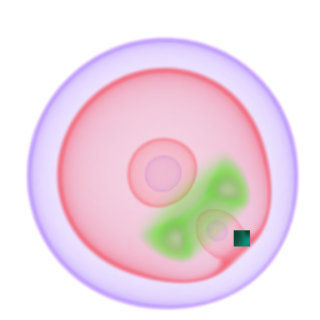
\includegraphics[width=1\linewidth]{nucleon_crop}\\
		(a)%\caption{Nucleon}
		\label{fig:nucleon}
	\end{minipage}~
	\begin{minipage}{.13\textwidth}
		\centering
		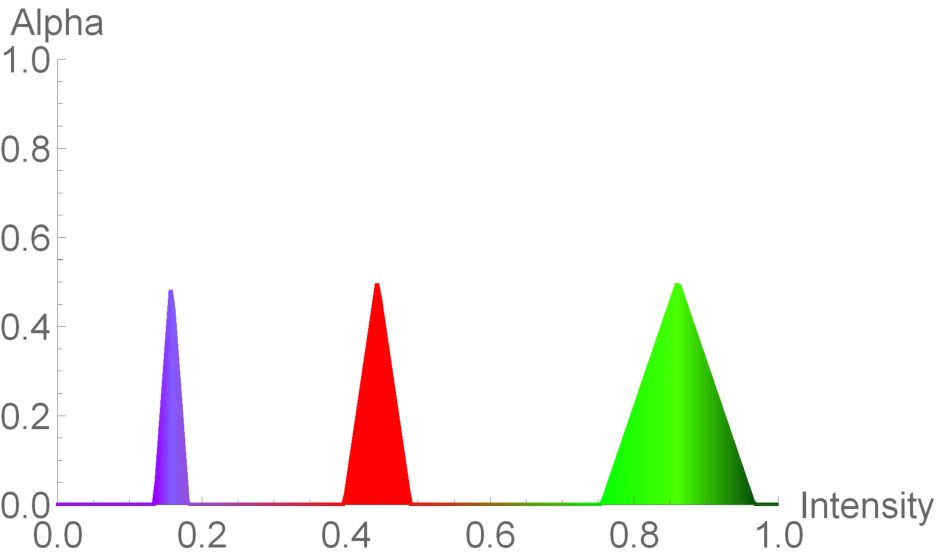
\includegraphics[width=1\linewidth]{tf_nucleon}\\
		(b)%\caption{TF of \autoref{fig:nucleon}}
		\label{fig:tf_nucleon}
	\end{minipage}~
	\begin{minipage}{.1\textwidth}
		\centering
		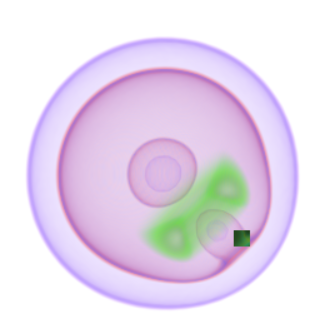
\includegraphics[width=1\linewidth]{nucleon_2_color_crop}
		(c)%\caption{Apply blue to \autoref{fig:nucleon}}
		\label{fig:nucleon_2_color}
	\end{minipage}~
	\begin{minipage}{.1\textwidth}
		\centering
		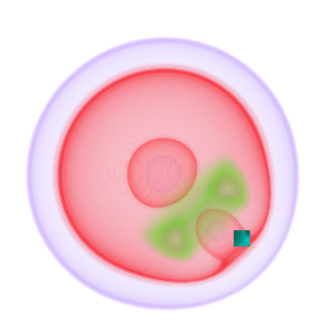
\includegraphics[width=1\linewidth]{nucleon_2_alpha_crop}
		(d)%\caption{Adjust alpha of \autoref{fig:nucleon}}
		\label{fig:nucleon_2_alpha}
	\end{minipage}
	%\caption{Example use case: (a) Nucleon data with small selected region (b) original transfer function;(c) Blue color applied to red region; (d) Alpha of red region adjusted	} 
	\caption{(a) Nucleon with a selected region; (b) TF of (a); (c) Blue applied to selected material; (d) opacity of selected material enhanced}
	\label{fig:nucleon_ori}
\end{figure}

\begin{figure}
	\centering
	\begin{minipage}{.155\textwidth}
		\centering
		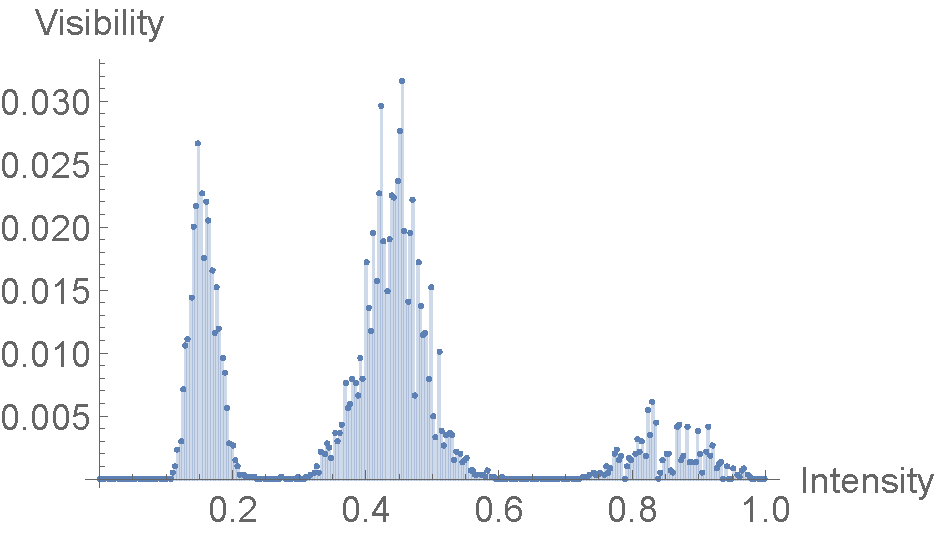
\includegraphics[width=1\linewidth]{global_visibility_histogram}
		(a)%\caption{Global visibility histogram}
		\label{fig:global_visibility_histogram}
	\end{minipage}~
	\begin{minipage}{.155\textwidth}
		\centering
		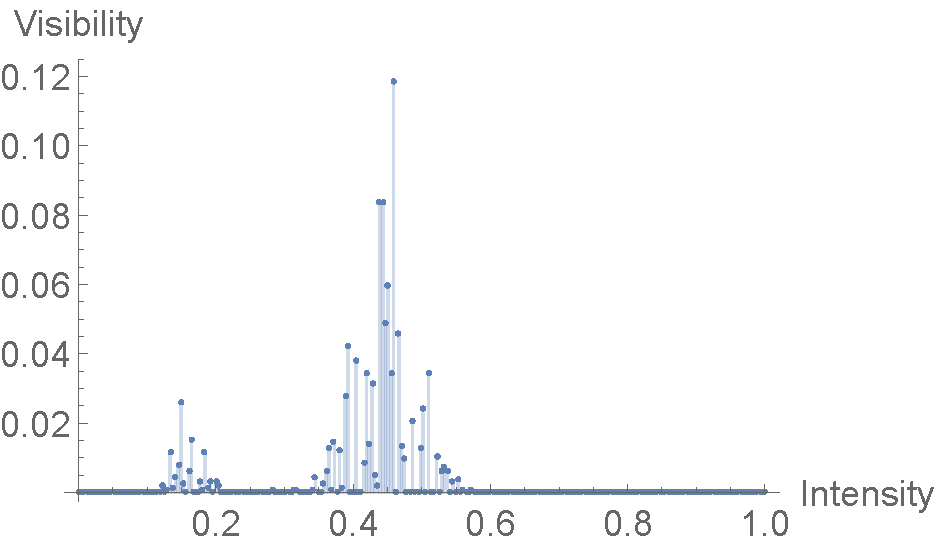
\includegraphics[width=1\linewidth]{local_visibility_histogram}
		(b)%		\caption{Local visibility histogram}
		\label{fig:local_visibility_histogram}
	\end{minipage}
	%\hspace{1cm}
	\begin{minipage}{.155\textwidth}
		\centering
		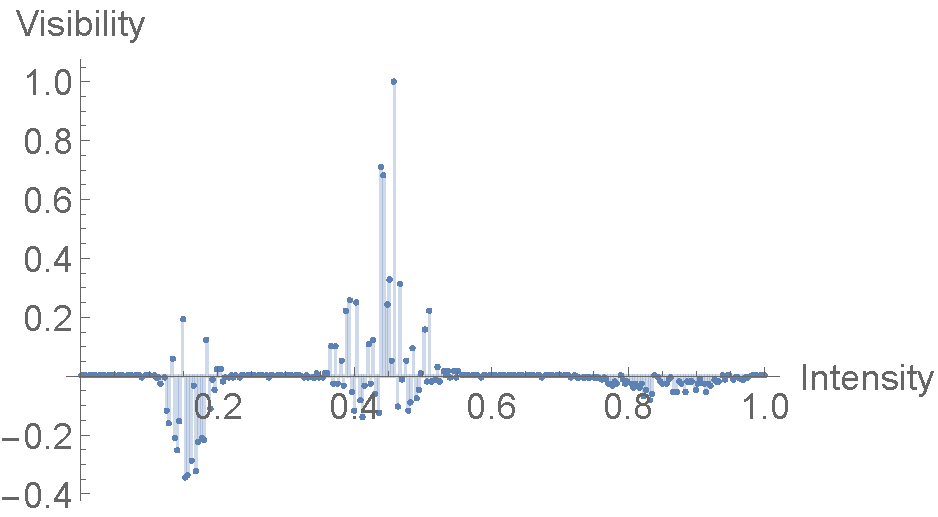
\includegraphics[width=1\linewidth]{relative_visibility_histogram}
		(c) %		\caption{Relative visibility histogram}
		\label{fig:relative_visibility_histogram}
	\end{minipage}~
	\begin{minipage}{.155\textwidth}
		\centering
		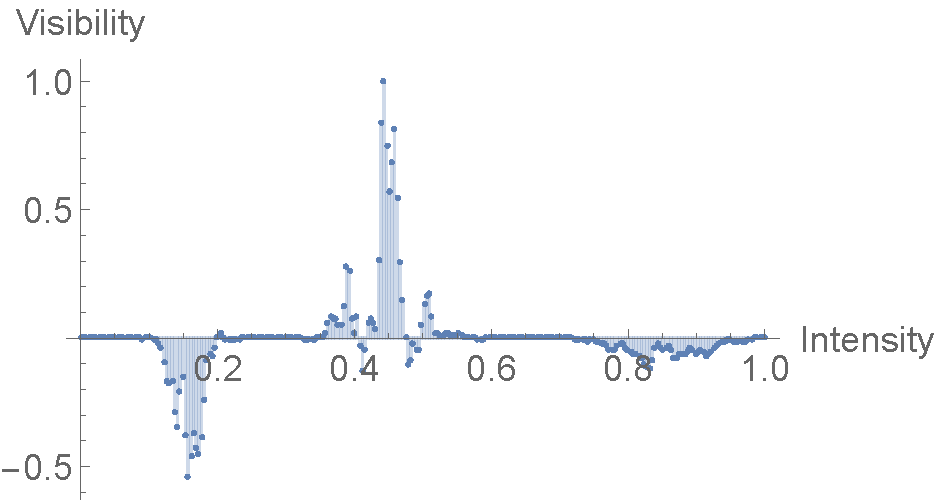
\includegraphics[width=1\linewidth]{relative_visibility_histogram_with_gaussian}
		(d) %		\caption{Smoothed relative visibility histogram}
		\label{fig:relative_visibility_histogram_with_gaussian}
	\end{minipage}
	\caption{(a) Global Visibility Histogram of dataset shown in \autoref{fig:nucleon_ori}(a); (b) Local Visibility Histogram of selected region; (c) Relative Visibility Histogram; (d) Relative visibility histogram after smoothing}
	\label{fig:nucleon_hist}
\end{figure}

\section{Relative Visibility Histograms}


A visibility histogram \cite{correa_visibility_2011} represents the visibility distribution of all voxels in the viewport when rendered from a given view, in other words how visible any voxel is, given its opacity and the degree to which it is occluded by other voxels in the view direction. We will use the more specific term \emph{Global visibility histogram}, $ H $, to describe such a distribution and define a subset of this, a \emph{Local visibility histogram}, $ H_{L} $,  as a histogram representating the local visibility distribution for the voxels that contribute to a region of interest (ROI) in the rendered image e.g. for a rectangular ROI on screen, this would be all the voxels that lie in the frustum extended by the rectangle. Furthermore we introduce the concept of a Relative Visibility Histogram, derived from the former which is defined as the difference between $ H_{L} $ and $ H $ divided by the maximum of the absolute value in the difference, i.e.
%$ H_{R}=H_{r}/max(abs(H_{r})) $, where $ H_{r}=H_{L}-H$.
\[
H_{R}=H_{r}/max(abs(H_{r}))
\]
where $ H_{r}=H_{L}-H$.
The relative visibility histogram is scaled to the range $ [-1,1] $ by dividing by the maximum absolute value in the histogram. 

The purpose of the relative visibility histogram is as follows: firstly the local $ H_L $ component captures the dominant intensities in the  region of interest. Secondly, the subtraction and normalization against the global context captures a representation of which intensities are particularly strongly distributed within the ROI and not elsewhere in the view. We posit that when a user selects any particular region of inte


An example is illustrated in Figure 1 and 2.
\autoref{fig:nucleon_ori} shows a nucleon data set, its associated transfer function and sample modifications using our technique.
The global visibility histogram is shown in 
\autoref{fig:nucleon_hist}(a) and the local visibility histogram for the region of interest (the rectangle in inverted color) is shown in \autoref{fig:nucleon_hist}(b). The relative visibility histogram
is show in \autoref{fig:nucleon_hist}(c).



%The relative visibility histogram in \autoref{fig:relative_visibility_histogram} is choppy, which is probably due to the small size of the selected region and some intensity values are missing.

%In order to get a smooth histogram for color and alpha blending, we apply a Gaussian kernel to $ H_{r} $ and then scale it to the range $ [-1,1] $.
In order to smooth the histogram, we apply a Gaussian kernel to $ H_{r} $ and then scale it to the range $ [-1,1] $.
So the smoothed relative visibility histogram is
%$ H_{G}= H_{g}/max(abs(H_{g}))$
\[ H_{G}= H_{g}/max(abs(H_{g})) \]
where $ H_{g}=Gaussian(H_{r},n,\sigma)$, $ n $ is the size and $ \sigma $ is the standard deviation of the Gaussian kernel (see \autoref{fig:nucleon_hist}(d)).

Henceforth, this smoothed histogram $ H_{G} $ will be referred to as the relative visibility histogram, and $ H_{G}(i) $, which is the value of the relative visibility histogram $ H_{G} $ at intensity $ i $, will be referred to as the relative visibility of intensity $ i$.




\begin{figure}
	\centering
	\begin{minipage}{.1\textwidth}
		\centering
		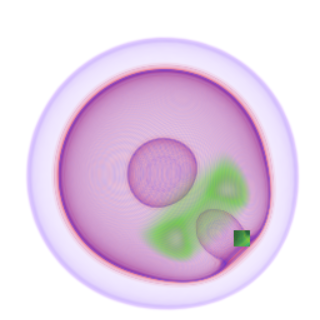
\includegraphics[width=1\linewidth]{nucleon_blue_crop}
		%\caption{Apply blue and adjust alpha of \autoref{fig:nucleon_ori}(a)}
		\label{fig:nucleon_2_blue}
	\end{minipage}~
	\begin{minipage}{.13\textwidth}
		\centering
		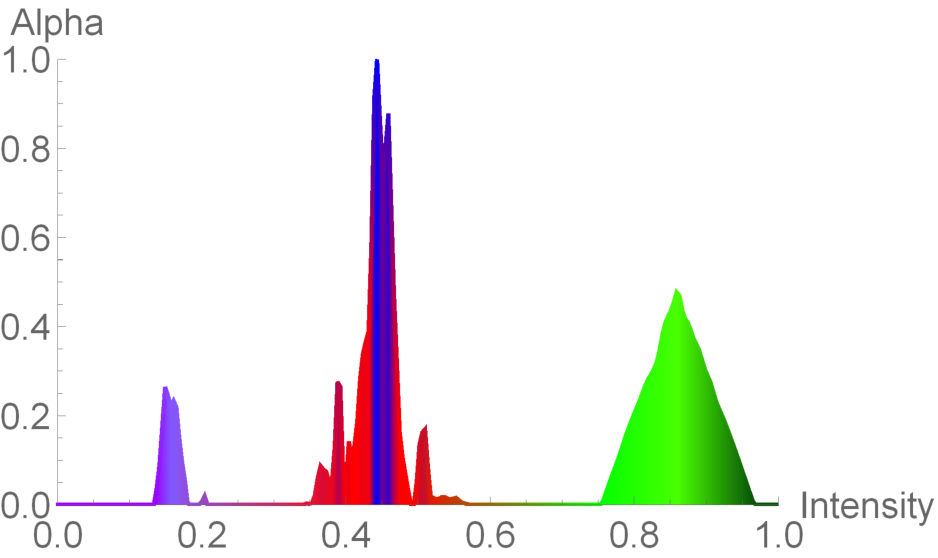
\includegraphics[width=1\linewidth]{tf_nucleon_2_blue}
		%\caption{TF of \autoref{fig:nucleon_2_blue}}
		\label{fig:tf_nucleon_2_blue}
	\end{minipage}~
	\begin{minipage}{.1\textwidth}
		\centering
		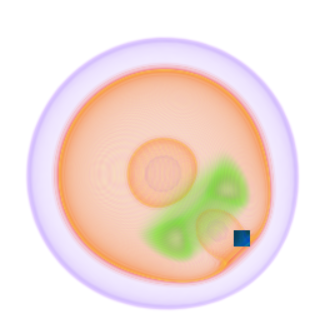
\includegraphics[width=1\linewidth]{nucleon_yellow_crop}
		%\caption{Apply yellow and adjust alpha of \autoref{fig:nucleon_ori}(a)}
		\label{fig:nucleon_2_yellow}
	\end{minipage}~
	\begin{minipage}{.13\textwidth}
		\centering
		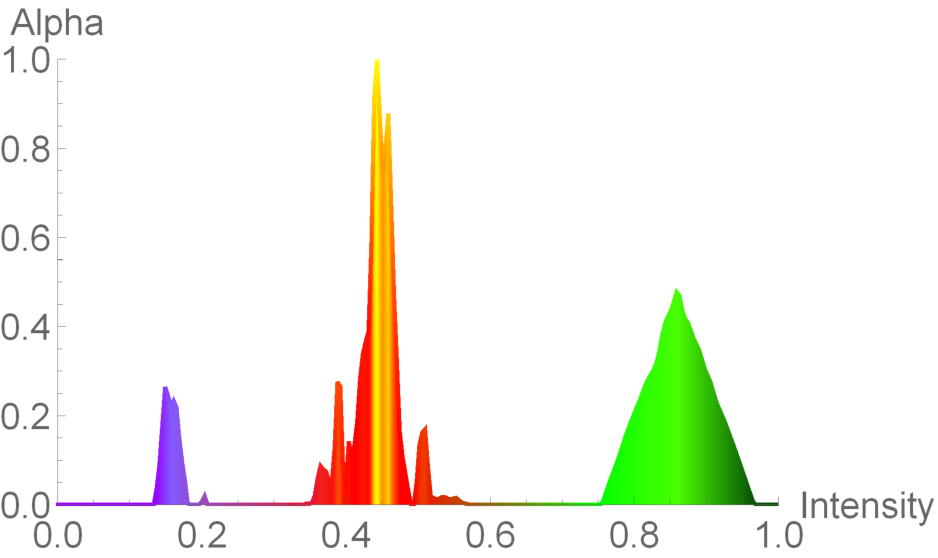
\includegraphics[width=1\linewidth]{tf_nucleon_2_yellow}
		%\caption{TF of \autoref{fig:nucleon_2_yellow}}
		\label{fig:tf_nucleon_2_yellow}
	\end{minipage}
	%	\begin{minipage}{.25\textwidth}
	%	\centering
	%	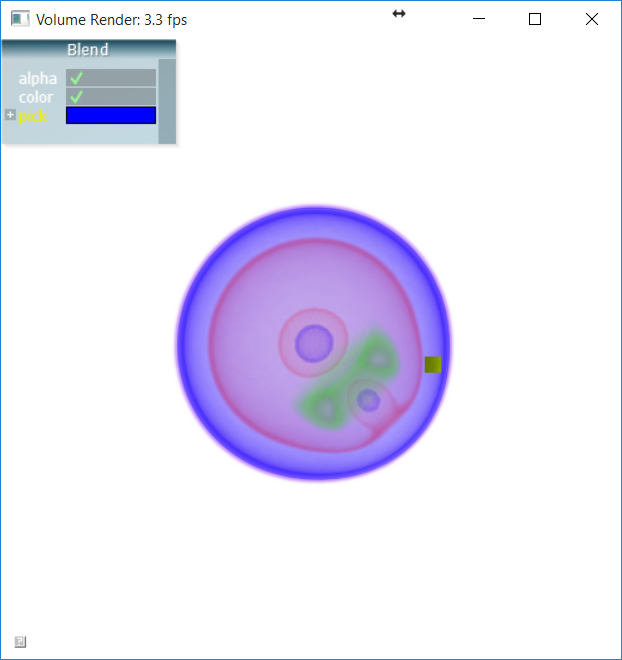
\includegraphics[width=1\linewidth]{nucleon_1_blue}
	%	\caption{Pick outside}
	%	\label{fig:nucleon_1_blue}
	%	\end{minipage}~
	%	\begin{minipage}{.25\textwidth}
	%	\centering
	%	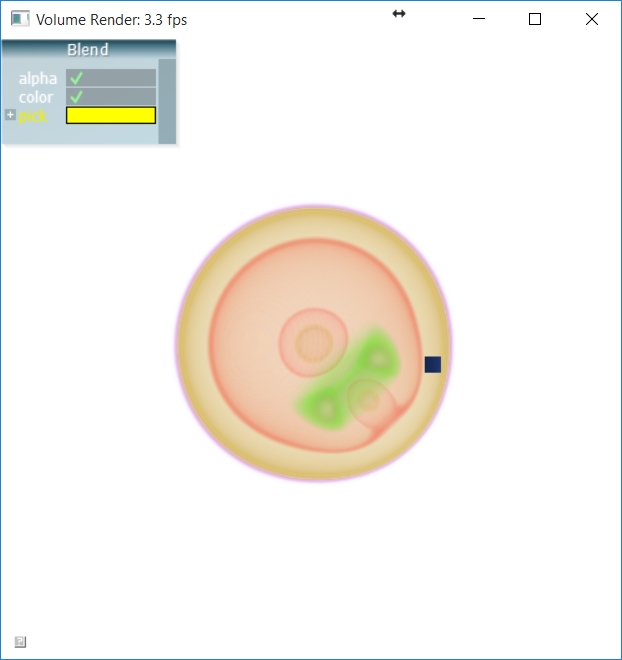
\includegraphics[width=1\linewidth]{nucleon_1_yellow}
	%	\caption{Pick outside}
	%	\label{fig:nucleon_1_yellow}
	%	\end{minipage}
	%		\begin{minipage}{.2\textwidth}
	%		\centering
	%		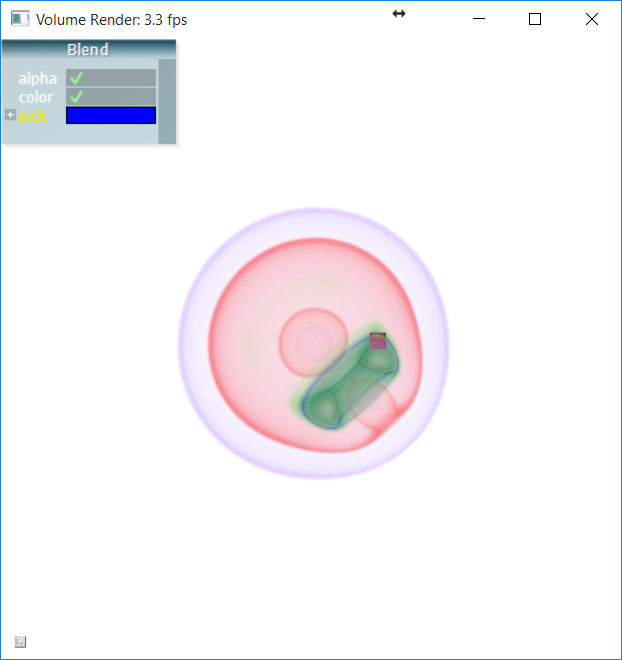
\includegraphics[width=1\linewidth]{nucleon_3_blue}
	%		\caption{Pick inside}
	%		\label{fig:nucleon_3_blue}
	%		\end{minipage}~
	%		\begin{minipage}{.2\textwidth}
	%		\centering
	%		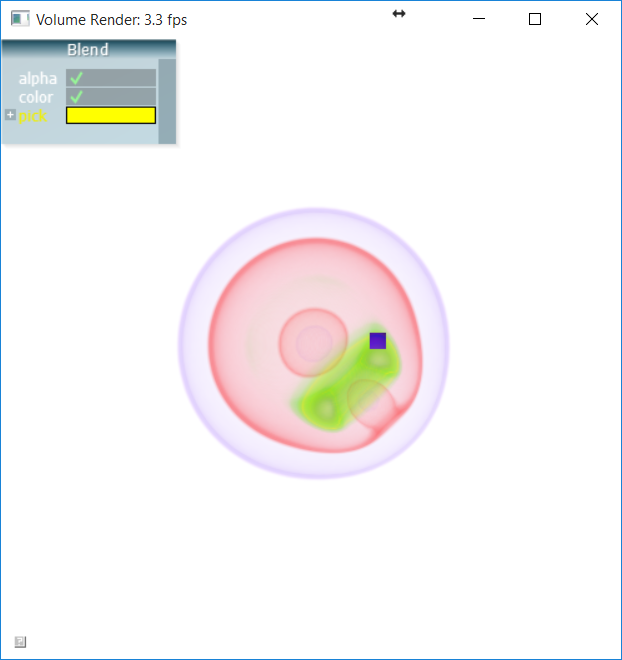
\includegraphics[width=1\linewidth]{nucleon_3_yellow}
	%		\caption{Pick inside}
	%		\label{fig:nucleon_3_yellow}
	%		\end{minipage}
	\caption{Left: Blue applied to selected region of TF in \autoref{fig:nucleon_ori}(b) and opacity enhanced; Right: Yellow applied and opacity enhanced. The modified TF is shown for each case alongside the rendering}
	\label{fig:Nucleon_2}
\end{figure}

%\section{Color and Alpha Blending}
%The color and alpha blending operations aim to provide an intuitive means for modifying and emphasizing visible materials of interest %based on the user preference information derived from the relative visibility histogram.
%The color blending applies a user-selected color to the intensity ranges with positive values in the relative visibility histogram, and the alpha blending increases the alpha of intensity ranges with positive relative visibility values and decreases the alpha of intensity ranges with negative relative visibility values.

%After the user has selected a region of interest on the volume rendering image, a pass of volume ray casting is done to calculate the global visibility histogram for the whole volume rendering image and the local visibility histogram for the selected region in the current view port. Subsequently, the relative visibility histogram is computed from the local and global visibility histograms for use in the color and alpha blending process.

%Let $ H_{G}(i) $ denote the relative visibility at intensity $ i $ in $ H_{G} $, $ C_{s} $ denote the user-selected color and $ C_{i} $ denote the color of intensity $ i $ in the transfer function.


\section{Color and Alpha Editing} \label{color_and_alpha_editing}

When a user selects a region of interest on the rendered image of the volume, a single pass of volume ray casting is done to calculate the global visibility histogram for the whole volume and the local visibility histogram for the selected region in the view-port. From this we calculate the relative visibility histogram, which provides a measure of visible materials within the selected region. This is used to infer features that the user intends to edit in the visualization. More precisely, $H_G$ is used as a weighting function to blend the colors or opacities in the original transfer function with a user-selected target color or alpha value.

The user-selected target color is blended with the original transfer function for intensity ranges that have positive values in the relative visibility histogram as below:
\[
C_{i} =
\begin{cases}
C_{i}+H_{G}(i)(C_{s}-C_{i}) & \text{if $ H_{G}(i)>0 $} \\
C_{i} & \text{otherwise}
\end{cases}
\]
where $ H_{G}(i) $ denotes the relative visibility at intensity $ i $ in $ H_{G} $, $ C_{s} $ is the user-selected target color and $ C_{i} $ the color of intensity $ i $ in the original transfer function.

Similarly, the alpha ($A_i$) of the transfer function is increased in intensity ranges that have positive relative visibility values, and decreased for ranges with negative relative visibility values, as follows:


%\[
%C_{i} =
%\begin{cases}
%C_{i}+H_{G}(i)(C_{s}-C_{i}) & \text{if $ H_{G}(i)>0 $} \\
%C_{i} & \text{otherwise}
%\end{cases}
%\]

%Similarly, let $ A_{i} $ denote the alpha of intensity $ i $. The alpha blending is

\[
A_{i} =
\begin{cases}
A_{i}+H_{G}(i)(1-A_{i}) & \text{if $ H_{G}(i)>0 $} \\
A_{i}-H_{G}(i)(0-A_{i}) & \text{otherwise}
\end{cases}
\]

Note that the color blending and alpha blending operations can be applied separately. \autoref{fig:nucleon_ori}(c) displays the result of only applying the color blending to the volume rendering of the nucleon data set in \autoref{fig:nucleon_ori}(a), and \autoref{fig:nucleon_ori}(d) displays the result of only applying the alpha blending to the original.

\section{Transfer Function Components} \label{transfer_function_components}
In addition to direct editing of the transfer function, we introduced transfer function components, which allow the user to edit the volume visualization on a feature level.

Ropinski et al. \cite{ropinski_stroke-based_2008} reported that physicians had high level requests such as emphasizing, adding or removing certain features in collaboratively adapting visualizations.

Relative visibility histograms reveal what intensity ranges are concentrated in the view frustum behind the selected region. Therefore, the visually dominant features in a selected region can be represented by component transfer functions proportional to the positive parts of relative visibility histograms.

The component transfer functions can be further composed into new transfer functions by modifying colors and opacity values of the components.

%This method allows the user to edit the volume visualization on a feature level.

%Relative visibility histograms represent the difference between the global visibility distribution across the full volume and the local visibility distribution within a user-selected region in the view port.

%The user can manipulate the colors and opacity values of the components and merge them to create new transfer functions.
%Automatically generate a component transfer function from a user-selected region.
%Combine the generated component transfer functions.

\subsection{Feature Specification Using Transfer Function Components}
In this approach, features are automatically generated as transfer function components based on the relative visibility histograms created from user-selected regions.
Let $F(i)$ denote a transfer function component derived from the relative visibility histogram $H_{G}$.
\[
F(i) =
\begin{cases}
H_{G}(i) & \text{if $ H_{G}(i)>0 $} \\
0 & \text{otherwise}
\end{cases}
\]

where $ H_{G}(i) $ is the value of the relative visibility histogram $ H_{G} $ at intensity $ i $.

\autoref{fig:nucleon_features} displays two transfer function components created from a green region and a red region in the volume rendering respectively.
\autoref{fig:nucleon_features} (a) and (b) show the two selected regions on the volume rendering. \autoref{fig:nucleon_features} (c) and (d) show the two transfer function components which represents the relative visibility distributions of features in the two user-selected regions respectively. Both regions are rectangles and the region sizes can be modified according to the user's need.

\subsection{Segments Selection with Image-Space Clustering}
Compared to selecting regions of geometric shapes, selecting visual objects in volume rendered images is more desirable for feature specification.
In order to achieve visual object selection, image segmentation is performed on volume rendered images and the resultant segments are stored in masks for object selection. More specifically, a GPU accelerated k-means clustering implementation is used to accomplish interactive segmentation of volume rendered images. The distance metric of the pixels is Euclidean distance in the RGB color space.

When the user clicks on a position of the volume rendered image, a selected region is formed by all pixels that belong to the same segment as the pixel at the mouse position.
\autoref{fig:nucleon_segments} displays the segments selected by clicking on the same screen positions as in \autoref{fig:nucleon_features}.

Compared to the rectangular regions in \autoref{fig:nucleon_features} (a) and (b), the selected regions in \autoref{fig:nucleon_segments} (a) and (b) are segments with colors similar to the pixels at the mouse positions. The regions in \autoref{fig:nucleon_segments} (a) and (b) are larger in sizes, which result in larger view frustums with more voxels being selected. Thus, the transfer function components in \autoref{fig:nucleon_segments} (c) and (d) are more continuous compared to those in \autoref{fig:nucleon_segments} (c) and (d). The relative visibility histograms in \autoref{fig:nucleon_segments} (e) and (f) are also smoother than those in \autoref{fig:nucleon_features} (e) and (f).

\begin{figure}
	\centering
	\begin{minipage}{.16\textwidth}
		\centering
		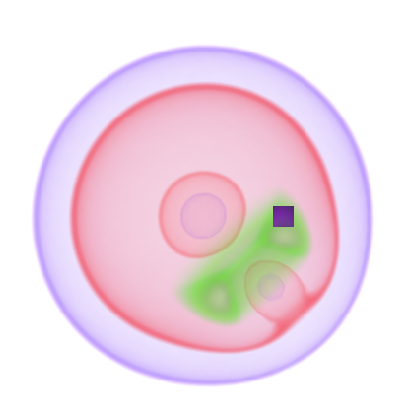
\includegraphics[width=1\linewidth]{crop/nucleon_selection_green}
(a)
	\end{minipage}~
	\begin{minipage}{.16\textwidth}
		\centering
		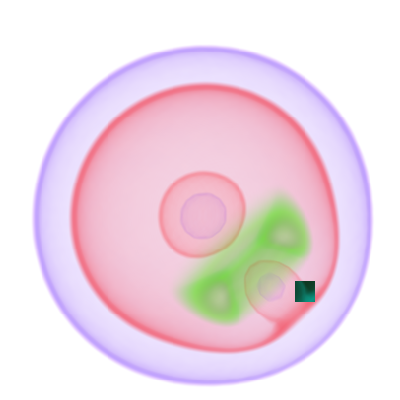
\includegraphics[width=1\linewidth]{crop/nucleon_selection_red}
(b)
	\end{minipage}
	\begin{minipage}{.16\textwidth}
	\centering
	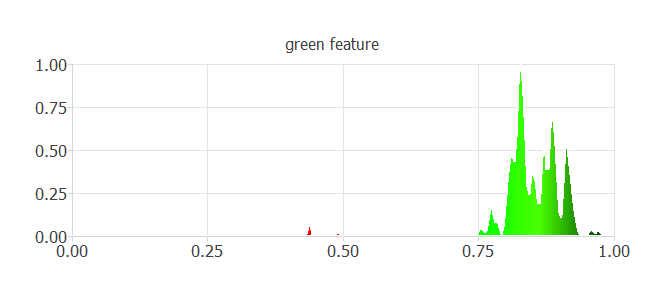
\includegraphics[width=1\linewidth]{nucleon_Green_feature}
(c)
	\end{minipage}~
	\begin{minipage}{.16\textwidth}
		\centering
		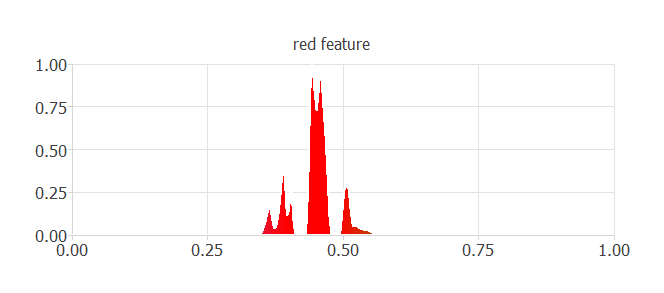
\includegraphics[width=1\linewidth]{nucleon_Red_feature}
(d)
	\end{minipage}
	\begin{minipage}{.16\textwidth}
		\centering
		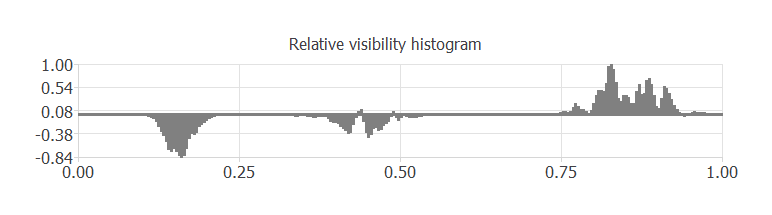
\includegraphics[width=1\linewidth]{nucleon_green_Relative_visibility_histogram}
(e)
	\end{minipage}~
	\begin{minipage}{.16\textwidth}
		\centering
		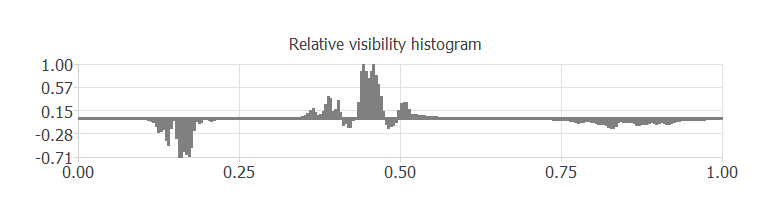
\includegraphics[width=1\linewidth]{nucleon_red_Relative_visibility_histogram}
(f)
	\end{minipage}
	\caption{Left: A TF component (c) created from a green region (a) (highlighted in inverted colors) and its relative visibility histogram (e); Right: A TF component (d) created from a red region (b) and its relative visibility histogram (f).}
	\label{fig:nucleon_features}
\end{figure}

\begin{figure}
	\centering
	\begin{minipage}{.16\textwidth}
		\centering
		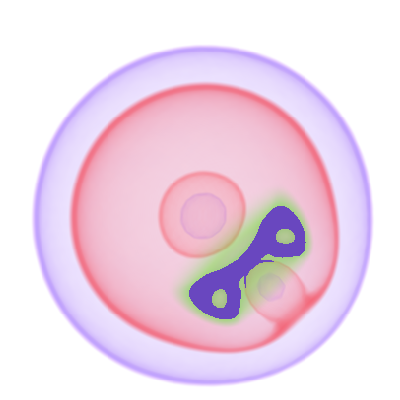
\includegraphics[width=1\linewidth]{crop/nucleon_segment_green}
(a)
	\end{minipage}~
	\begin{minipage}{.16\textwidth}
		\centering
		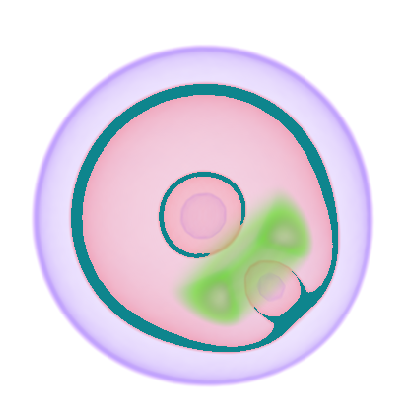
\includegraphics[width=1\linewidth]{crop/nucleon_segment_red}
(b)
	\end{minipage}
	\begin{minipage}{.16\textwidth}
		\centering
		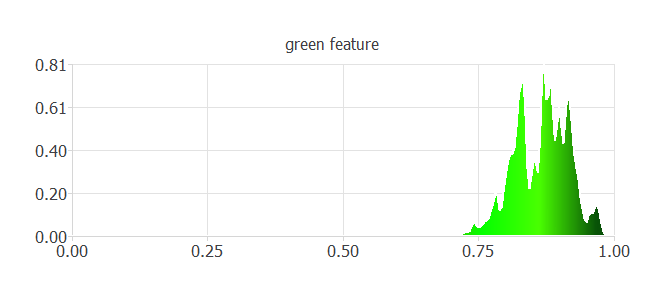
\includegraphics[width=1\linewidth]{nucleon_green_segment}
(c)
	\end{minipage}~
	\begin{minipage}{.16\textwidth}
		\centering
		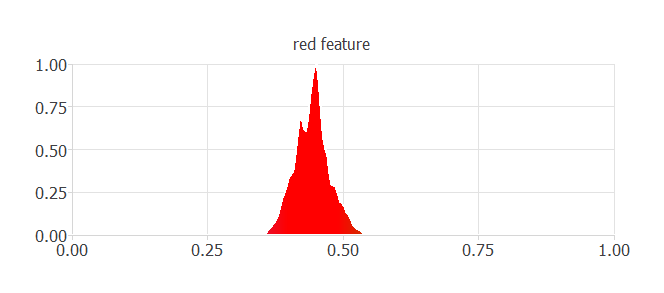
\includegraphics[width=1\linewidth]{nucleon_red_segment}
(d)
	\end{minipage}
	\begin{minipage}{.16\textwidth}
		\centering
		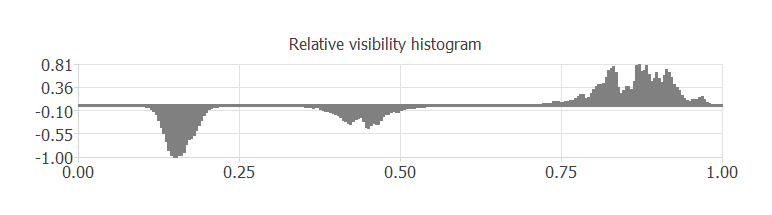
\includegraphics[width=1\linewidth]{nucleon_green_segment_Relative_visibility_histogram}
(e)
	\end{minipage}~
	\begin{minipage}{.16\textwidth}
		\centering
		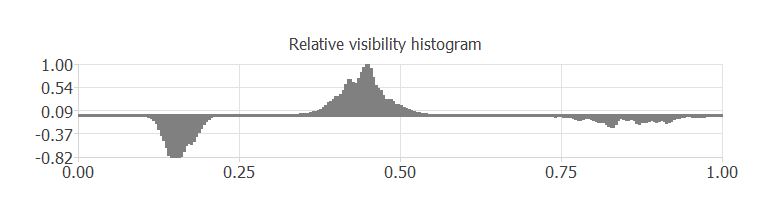
\includegraphics[width=1\linewidth]{nucleon_red_segment_Relative_visibility_histogram}
(f)
	\end{minipage}
	\caption{Left: A TF component (c) created from a green segment (a) (highlighted in inverted colors) and its relative visibility histogram (e); Right: A TF component (d) created from a red segment (b) and its relative visibility histogram (f).}
	\label{fig:nucleon_segments}
\end{figure}

\begin{figure}
	\centering
	\begin{minipage}{.16\textwidth}
		\centering
		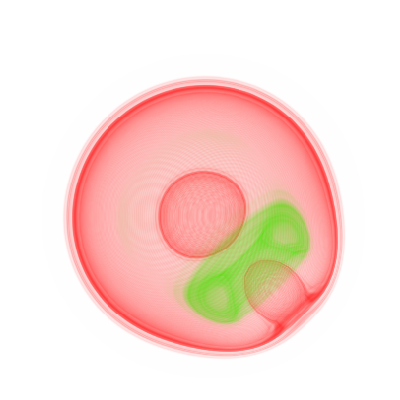
\includegraphics[width=1\linewidth]{crop/nucleon_merged_green_red}
		(a)
	\end{minipage}~
	\begin{minipage}{.16\textwidth}
		\centering
		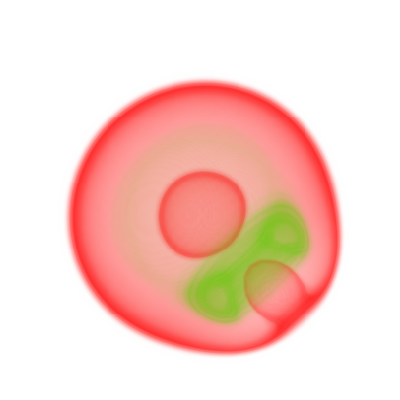
\includegraphics[width=1\linewidth]{crop/nucleon_merged_segment_green_red}
		(b)
	\end{minipage}
	\begin{minipage}{.16\textwidth}
		\centering
		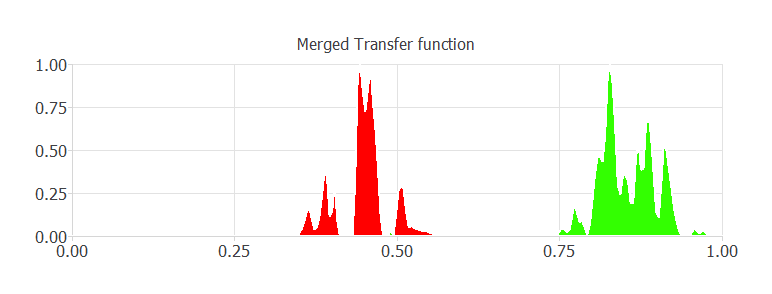
\includegraphics[width=1\linewidth]{nucleon_green_red_Merged_Transfer_function}
		(c)
%	\caption{nucleon_merged_green_red}
%	\label{fig:nucleon_merged_green_red}
	\end{minipage}~
	\begin{minipage}{.16\textwidth}
		\centering
		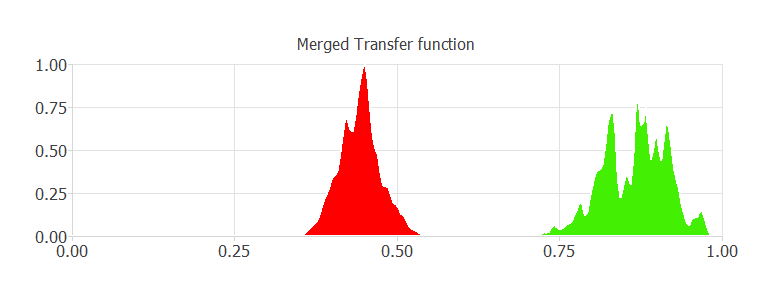
\includegraphics[width=1\linewidth]{nucleon_green_red_segment_Merged_Transfer_function}
		(d)
%	\caption{nucleon_merged_segment_green_red}
%	\label{fig:nucleon_merged_segment_green_red}
	\end{minipage}
	\caption{(a) and (c): Volume rendering and its TF from merging the TF components in \autoref{fig:nucleon_features}; (b) and (d): Volume rendering and its TF from merging the TF components in \autoref{fig:nucleon_segments}}
	\label{fig:nucleon_merged}
\end{figure}

%\begin{figure}
%	\centering
%	\begin{minipage}{.16\textwidth}
%		\centering
%		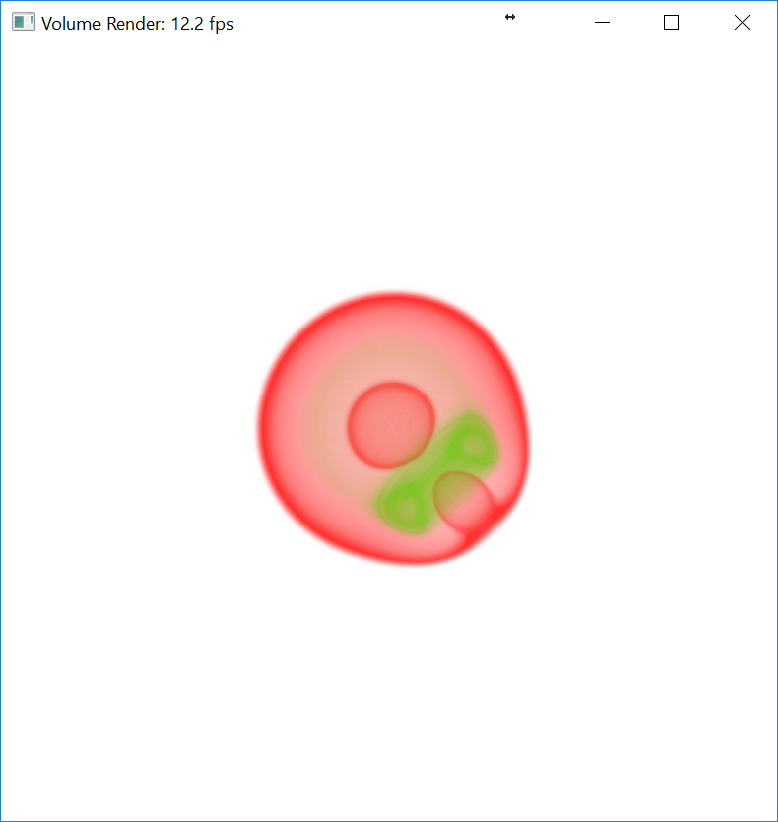
\includegraphics[width=1\linewidth]{nucleon_merged_segment_green_red}
%	\end{minipage}~
%	\begin{minipage}{.16\textwidth}
%		\centering
%		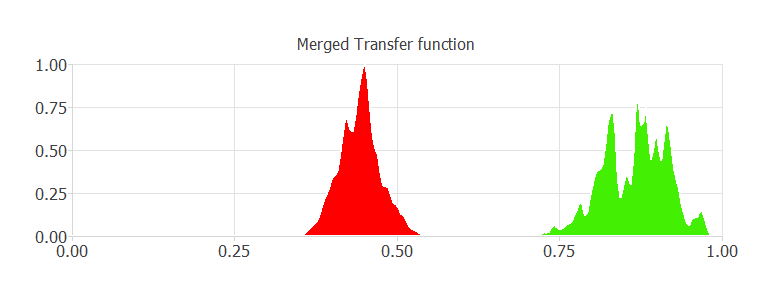
\includegraphics[width=1\linewidth]{nucleon_green_red_segment_Merged_Transfer_function}
%	\end{minipage}
%	\caption{Left: Create TF component from a green region (the region is highlighted in inverted color); Middle: Create component from a red region; Right: Create component from a purple region}
%	\label{fig:nucleon_merged_segments}
%\end{figure}

\subsection{Merging Transfer Function Components}
A new transfer function can be created by merging several transfer function components.

The opacity function $ A_{i} $ is defined by a weighted sum of transfer function components clipped to the range $ [0,1] $.

\[
A_{i} =
\begin{cases}
a(i) & \text{if $ a(i) \in [0,1] $} \\
0 & \text{if $ a(i)<0 $} \\
1 & \text{if $ a(i)>1 $}
\end{cases}
\]

where $ a(i) $ is the weighted sum of transfer function components, i.e.

\[ 
a(i)=\sum_{j=1}^{n} w_{j}F_{j}(i)
\]

where $ w_{j} $ ($ w_{j} \geq 0 $) is the weight for transfer function component $ F_{j} $, $ F_{j}(i) $ is the value of $ F_{j} $ at intensity $ i $, and $ n $ is the number of transfer function components.

\autoref{fig:nucleon_merged} shows the results of merging the transfer function components in \autoref{fig:nucleon_features} and \autoref{fig:nucleon_segments} respectively.

Note that there are ``wood grain'' artifacts in the volume rendered image in \autoref{fig:nucleon_merged} (a), especially in the red feature. The artifacts are due to the gaps in the transfer function components, as shown in \autoref{fig:nucleon_merged} (c).
In contrast, the volume rendered image in \autoref{fig:nucleon_merged} (b) does not has noticeable artifacts, because the transfer function components in \autoref{fig:nucleon_merged} (d) are smoother.

There may be overlaps between transfer function components. Two methods for deciding the color of the overlaps in the merged transfer functions are described below.

\subsubsection{Blending colors of transfer function components}
The first method is blending the colors of the transfer function components based on the weights and the values of the transfer function components.

In order to keep the blended colors in a valid range, the weights for blending the colors of transfer function components are normalized using weighted averages of the weights and the values of the transfer function components.
The normalized weight of transfer function component $ F_{j} $ is defined by
\[ W_{j}=
\frac{w_{j}F_{j}(i)}{\sum_{k=1}^{n}w_{k}F_{k}(i)}
\]
where $ w_{j} $ ($ w_{j} \geq 0 $) is the weight of transfer function component $ F_{j} $, $ F_{k}(i) $ is the value of the transfer function component $ F_{k} $ at intensity $ i $, and $ n $ is the number of transfer function components.

Hence, the color function $ C_{i} $ is defined by
\[ C_{i}=
\sum_{j=1}^{n} W_{j}c_{j}
\]
where $ W_{j} $ is the normalized weight of transfer function component $ F_{j} $ and $ c_{j} $ is the color of $ F_{j} $, and $ n $ is the number of transfer function components.

Using this color blending method, new colors that do not exist in the settings of transfer function components may be introduced due to the blending of colors of overlapping transfer function components.
Moreover, a feature, represented by a transfer function component, may have various colors in the volume rendering.

\subsubsection{Using colors of the dominant components}
In some cases, using a single color for a feature is preferable for better distinction of features in the volume rendering.

The second method is using the color of the visually dominant transfer function component as the merged color.

The color function $ C_{i} $ is defined by
\[ 
C_{i} = c_{j},\quad j = \argmax_{k \in \{1,...,n\}} w_{k}F_{k}(i)
\]
where $ c_{j} $ is the color and $ w_{j} $ ($ w_{j} \geq 0 $) is the weight of transfer function component $ F_{j} $ with $ w_{j}F_{j}(i) $ at intensity $ i $ that is maximum among the $ n $ transfer function components.

With this method, different features would have distinct colors, so that they are distinguishable by colors in the volume rendering.

\section{Results}

We have implemented our approach with a GPU-Raycast volume renderer with the visibility computation and rendering implemented on a GPU using CUDA. The implementation is quite lightweight, and achieves real-time performance at 36 to 40 frames per second on a computer equipped with an Intel Xeon E3-1246 v3 CPU and a NVIDIA Quadro K4200 graphics card.
%When the color and alpha blending is performed on a user-selected region, the first pass of volume ray-casting is done to calculate the global and local visibility histograms and the volume is rendered in the second pass of ray-casting using the transfer function from the blending result.

\subsection{Direct Transfer Function Editing}

\autoref{fig:Nucleon_2}(left) displays the result of both applying color blue and adjusting alpha of the TF in \autoref{fig:nucleon_ori}(b). Note that the intensity ranges with initial red color in the middle of the transfer function have been blended with blue and have become purple.
Similarly, \autoref{fig:Nucleon_2}(right) shows the result of applying yellow and adjusting alpha. Here, the intensity ranges in the middle have become orange after blending with the color yellow. 
In both cases, the alpha of the relevant parts of the transfer function are increased and the alpha of the less relevant parts are decreased in order to emphasize the materials of interest.

Figure \ref{fig:CT-knee_all}(left) shows show a rendered image of a CT-Knee dataset with a selected region over the bone. Figure \ref{fig:CT-knee_all}(right) shows the image and the transfer function after applying a blue color and alpha adjustment. The bone material becomes mostly blue and is emphasized due to increased opacity, whilst the materials around the bone with lower relative intensity ranges are de-emphasized.

Figure \ref{fig:Vortex_all} shows results of enhancing one time-step of a turbulent vortex data set.
\autoref{fig:Vortex_all}(a) shows the rendered image and original transfer function.
\autoref{fig:Vortex_all}(b) shows a clear visualization, and respective TF, of the materials of interest blended with blue and emphasized with higher alpha.
Similarly, \autoref{fig:Vortex_all}(c) shows the materials of interest blended with yellow and emphasized with higher alpha.

The examples show that the technique can be applied effectively to a range of different datasets and transfer functions. Although we only show single step examples due to space constraints, it should be suitable for iterative editing such as in a paintbrush like tool for a large number successive of operations.

\begin{figure}
	\centering
	\begin{minipage}{.1\textwidth}
		\centering
		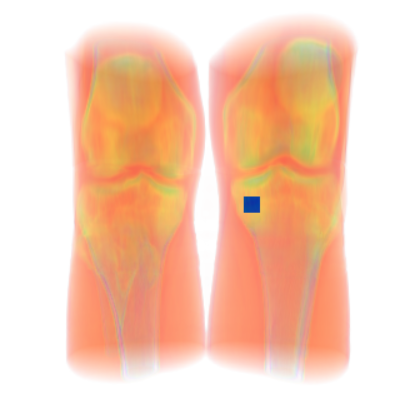
\includegraphics[width=1\linewidth]{CT-Knee_crop}
		%\caption{CT-Knee}
		\label{fig:CT-Knee}
	\end{minipage}~
	\begin{minipage}{.12\textwidth}
		\centering
		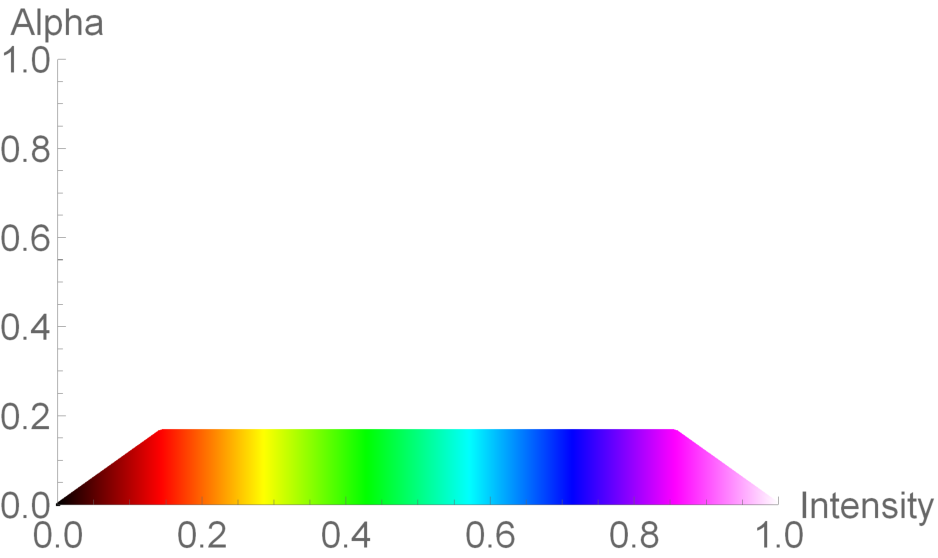
\includegraphics[width=1\linewidth]{tf_CT-Knee}
		%\caption{TF of \autoref{fig:CT-Knee}}
		\label{fig:tf_CT-Knee}
	\end{minipage}~
	\begin{minipage}{.1\textwidth}
		\centering
		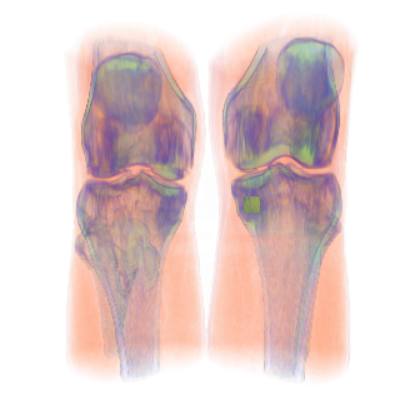
\includegraphics[width=1\linewidth]{CT-Knee_blue_crop}
		%\caption{Apply blue and adjust alpha of \autoref{fig:CT-Knee}}
		\label{fig:CT-Knee_blue}
	\end{minipage}~
	\begin{minipage}{.12\textwidth}
		\centering
		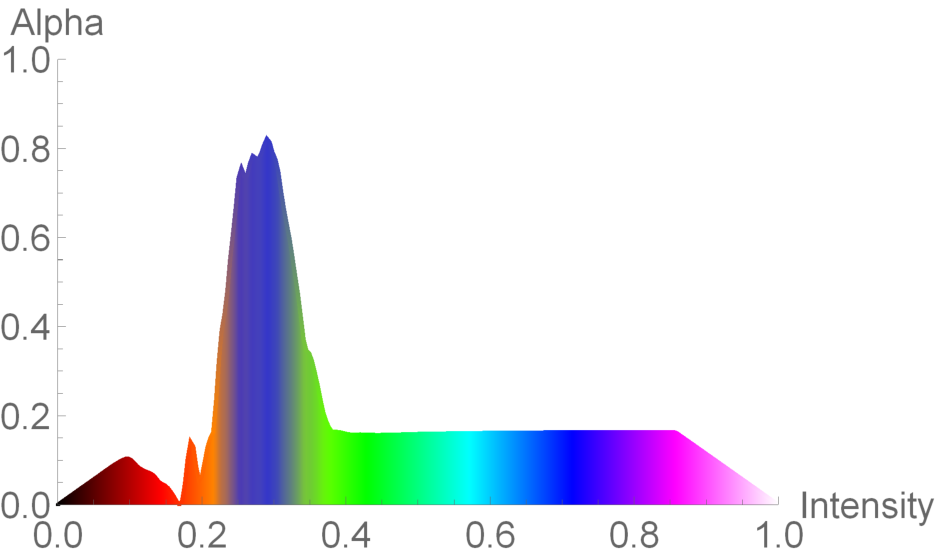
\includegraphics[width=1\linewidth]{tf_CT-Knee_blue}
		%\caption{TF of \autoref{fig:CT-Knee_blue}}
		\label{fig:tf_CT-Knee_blue}
	\end{minipage}
	\caption{Left: CT-Knee dataset and basic TF; Right: Blue applied and opacity enhanced for selected region}
	\label{fig:CT-knee_all}
	
\end{figure}

\begin{figure}
	\centering
	\begin{minipage}{.14\textwidth}
		\centering
		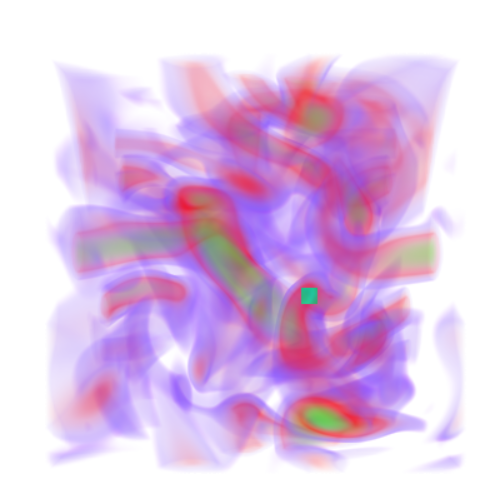
\includegraphics[width=1\linewidth]{vortex_crop}
		%\caption{Vortex}
		\label{fig:vortex}
	\end{minipage}~
	\begin{minipage}{.14\textwidth}
		\centering
		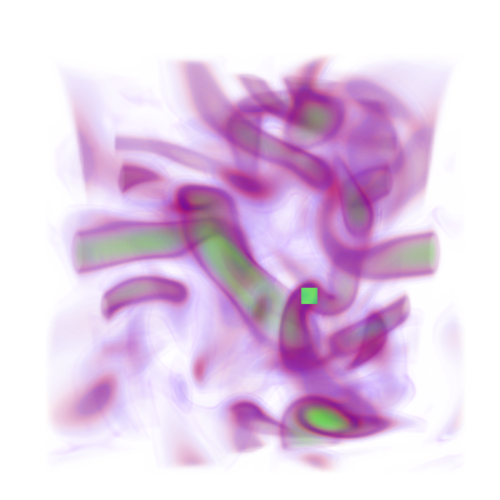
\includegraphics[width=1\linewidth]{vortex_blue_crop}
		%\caption{Apply blue and adjust alpha of \autoref{fig:vortex}}
		\label{fig:vortex_2_blue}
	\end{minipage}~
	\begin{minipage}{.14\textwidth}
		\centering
		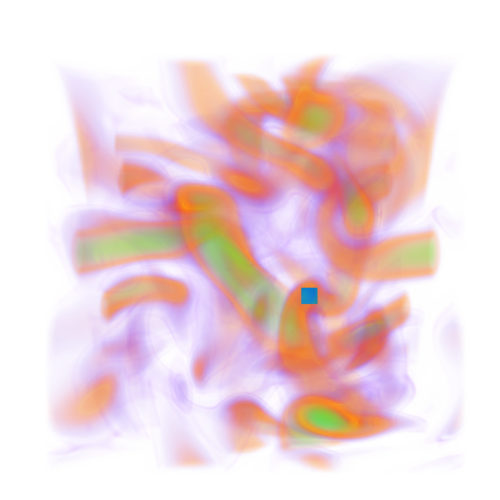
\includegraphics[width=1\linewidth]{vortex_yellow_crop}
		%\caption{Apply yellow and adjust alpha of \autoref{fig:vortex}}
		\label{fig:vortex_2_yellow}
	\end{minipage}
	\begin{minipage}{.16\textwidth}
		\centering
		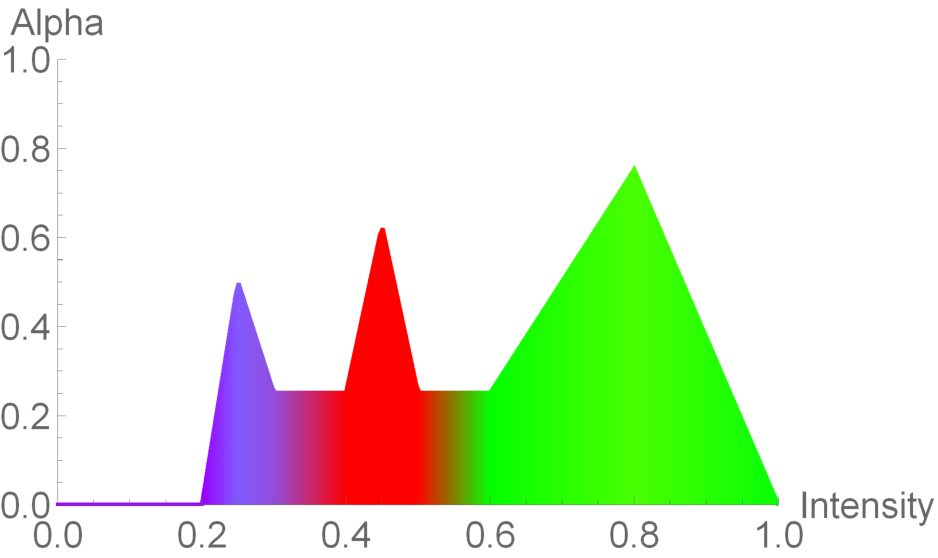
\includegraphics[width=.91\linewidth]{tf_vortex}
		(a)%\caption{TF of \autoref{fig:vortex}}
		\label{fig:tf_vortex}
	\end{minipage}~
	\begin{minipage}{.16\textwidth}
		\centering
		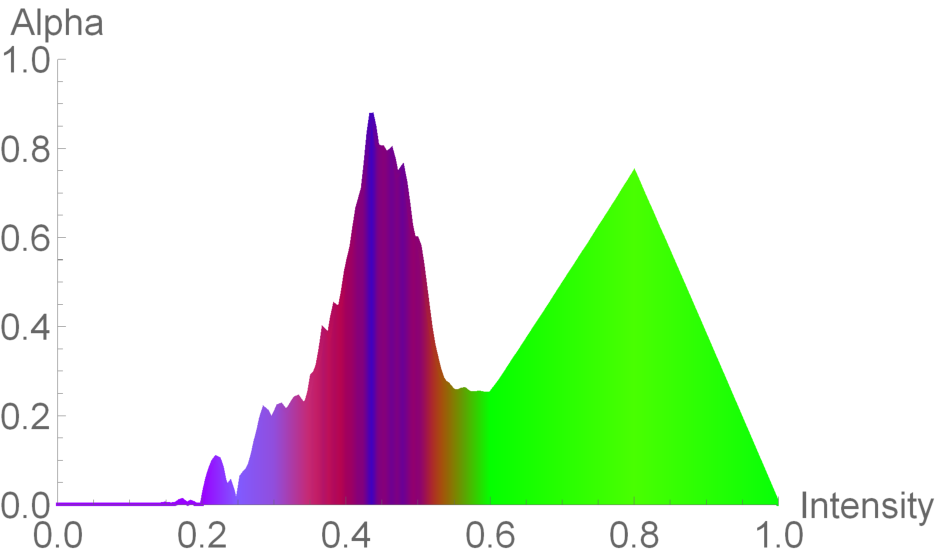
\includegraphics[width=.91\linewidth]{tf_vortex_2_blue}
		(b)%\caption{TF of \autoref{fig:vortex_2_blue}}
		\label{fig:tf_vortex_2_blue}
	\end{minipage}~
	\begin{minipage}{.16\textwidth}
		\centering
		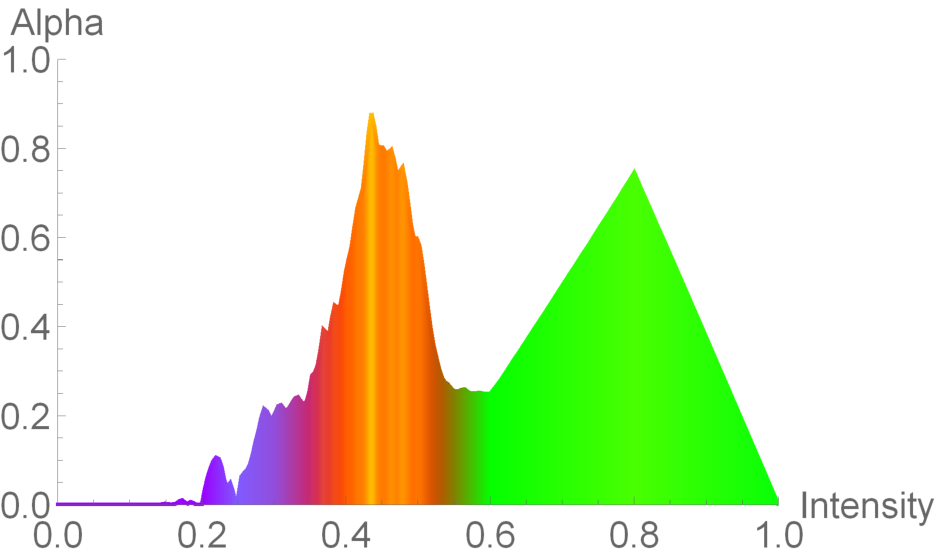
\includegraphics[width=.91\linewidth]{tf_vortex_2_yellow}
		(c)%\caption{TF of \autoref{fig:vortex_2_yellow}}
		\label{fig:tf_vortex_2_yellow}
	\end{minipage}
	%\begin{minipage}{.2\textwidth}
	%	\centering
	%	\includegraphics[width=1\linewidth]{vortex_3_blue}
	%	\caption{vortex blue}
	%	\label{fig:vortex_3_blue}
	%\end{minipage}~
	%\begin{minipage}{.2\textwidth}
	%	\centering
	%	\includegraphics[width=1\linewidth]{vortex_3_yellow}
	%	\caption{vortex yellow}
	%	\label{fig:vortex_3_yellow}
	%\end{minipage}
	\caption{(a)Turbulent vortex dataset and initial TF; (b)Blue applied to selected material and opacity enhanced; (c) Yellow applied and opacity enhanced.}
	\label{fig:Vortex_all}
\end{figure}


%\autoref{fig:nucleon_features} displays two transfer function components created from a green region and a red region in the volume rendering respectively.
%\autoref{fig:nucleon_features} (a) and (b) show the two selected regions on the volume rendering. \autoref{fig:nucleon_features} (c) and (d) show the two transfer function components which represents the relative visibility distributions of features in the two user-selected regions respectively. Both user-selected regions are rectangular and the region sizes can be modified according to the user's need.

\subsection{TF-components editing}
\autoref{fig:vortex_features}, \autoref{fig:vortex_segments}, \autoref{fig:vortex_merged} and \autoref{fig:vortex_merged_2} show results of creating and merging transfer function components on the time-step of the turbulent vortex data set.

\autoref{fig:vortex_features} displays three transfer function components created from a green region, a red region and a purple region, which are rectangular regions highlighted in inverted colors, in the volume rendering respectively.
In contrast, \autoref{fig:vortex_segments} displays three transfer function components created from three regions based on image segmentation results. The three regions are visual objects with similar colors and are selected by clicking on the same positions as in the regions in \autoref{fig:vortex_features}.

\autoref{fig:vortex_merged} (a) and (d) show the volume rendered image and the transfer function created from merging the three transfer function components in \autoref{fig:vortex_features}.
Similarly, \autoref{fig:vortex_merged} (b) and (e) display the volume rendered image and the transfer function created from merging the three transfer function components in \autoref{fig:vortex_segments} with color blending, and \autoref{fig:vortex_merged} (c) and (f) display the results of merging the three transfer function components in \autoref{fig:vortex_segments} using colors of dominant components.
In \autoref{fig:vortex_merged}, the three transfer function components are merged with weights \{2,1,0.2\}, so that the purple feature is de-emphasized, the green feature is emphasized, and the red feature remains the same level of opacity.

We observed that the transfer function components in \autoref{fig:vortex_merged} (e) and (f), which are derived from segments, have wider intensity ranges than those in \autoref{fig:vortex_merged} (d), which are derived from rectangular regions.

\autoref{fig:vortex_merged_2} displays the results of merging two transfer function components, i.e. the green feature and the red feature, with weights \{2,1\} and setting the colors of the two components to blue and orange respectively.

\begin{figure}
	\centering
	\begin{minipage}{.16\textwidth}
		\centering
		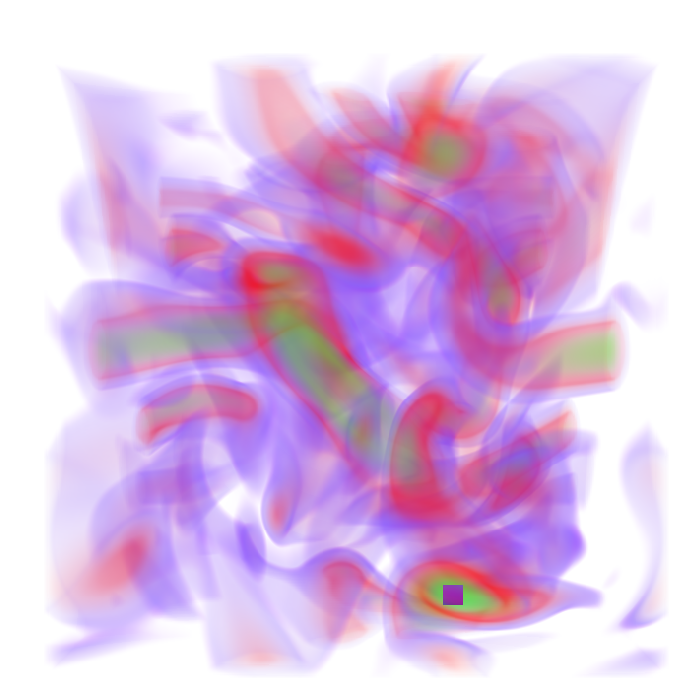
\includegraphics[width=1\linewidth]{crop/vortex_selection_green}
		(a)
	\end{minipage}~
	\begin{minipage}{.16\textwidth}
		\centering
		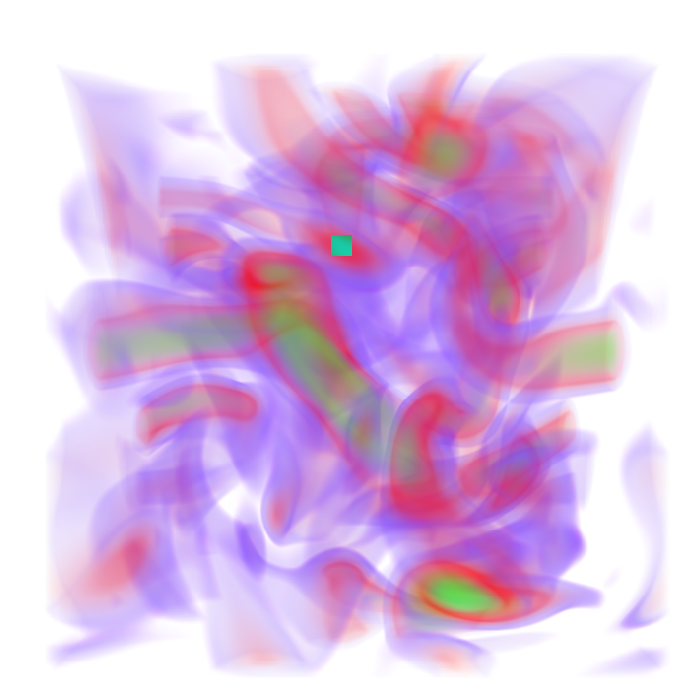
\includegraphics[width=1\linewidth]{crop/vortex_selection_red}
		(b)
	\end{minipage}~
	\begin{minipage}{.16\textwidth}
		\centering
		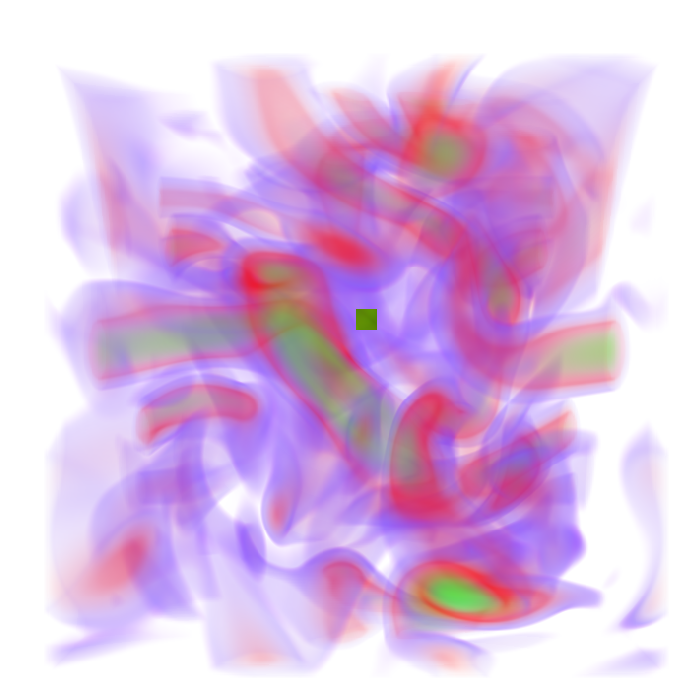
\includegraphics[width=1\linewidth]{crop/vortex_selection_purple}
		(c)
	\end{minipage}
	\caption{User-selected regions highlighted in inverted colors. (a): a rectangular region in the green material; (b): a rectangular region in the red material; (c): a rectangular region in the purple material}
	\label{fig:vortex_features}
\end{figure}

\begin{figure}
	\centering
	\begin{minipage}{.16\textwidth}
		\centering
		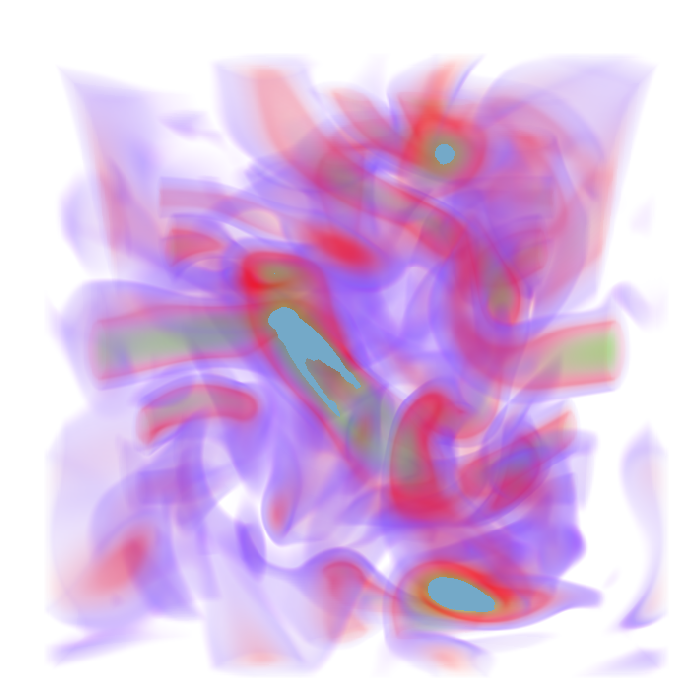
\includegraphics[width=1\linewidth]{crop/vortex_segment_green}
		(a)
	\end{minipage}~
	\begin{minipage}{.16\textwidth}
		\centering
		\includegraphics[width=1\linewidth]{crop/vortex_segment_red}
		(b)
	\end{minipage}~
	\begin{minipage}{.16\textwidth}
		\centering
		\includegraphics[width=1\linewidth]{crop/vortex_segment_purple}
		(c)
	\end{minipage}
	\caption{User-selected segments highlighted in inverted colors. (a): a segment in the green material; (b): a segment in the red material; (c): a segment in the purple material}
	\label{fig:vortex_segments}
\end{figure}

\begin{figure}
	\centering
	\begin{minipage}{.16\textwidth}
		\centering
		\includegraphics[width=1\linewidth]{crop/vortex_merged_green_red_purple}
		(a)
	\end{minipage}~
	\begin{minipage}{.16\textwidth}
		\centering
		\includegraphics[width=1\linewidth]{crop/vortex_merged_segment_blend_green_red_purple}
		(b)
	\end{minipage}~
	\begin{minipage}{.16\textwidth}
		\centering
		\includegraphics[width=1\linewidth]{crop/vortex_merged_segment_green_red_purple}
		(c)
	\end{minipage}
	\begin{minipage}{.16\textwidth}
		\centering
		\includegraphics[width=1\linewidth]{tf_vortex_merged_green_red_purple}
		(d)
	\end{minipage}~
	\begin{minipage}{.16\textwidth}
		\centering
		\includegraphics[width=1\linewidth]{tf_vortex_merged_segment_blend_green_red_purple}
		(e)
	\end{minipage}~
	\begin{minipage}{.16\textwidth}
		\centering
		\includegraphics[width=1\linewidth]{tf_vortex_merged_segment_green_red_purple}
		(f)
	\end{minipage}
	\caption{Merge 3 features with weights \{2,1,0.2\}; (a) and (d): Volume rendering and TF from merging the TF components in \autoref{fig:vortex_features}; (b) and (e): Volume rendering and TF from merging the TF components in \autoref{fig:vortex_segments} with color blending; (c) and (f): Volume rendering and TF from merging the TF components in \autoref{fig:vortex_segments} using colors of dominant components}
	\label{fig:vortex_merged}
\end{figure}

\begin{figure}
	\centering
	\begin{minipage}{.16\textwidth}
		\centering
		\includegraphics[width=1\linewidth]{crop/vortex_merged_green_red}
		(a)
	\end{minipage}~
	\begin{minipage}{.16\textwidth}
		\centering
		\includegraphics[width=1\linewidth]{crop/vortex_merged_segment_blend_green_red}
		(b)
	\end{minipage}~
	\begin{minipage}{.16\textwidth}
		\centering
		\includegraphics[width=1\linewidth]{crop/vortex_merged_segment_green_red}
		(c)
	\end{minipage}
	\begin{minipage}{.16\textwidth}
		\centering
		\includegraphics[width=1\linewidth]{tf_vortex_merged_green_red}
		(d)
	\end{minipage}~
	\begin{minipage}{.16\textwidth}
		\centering
		\includegraphics[width=1\linewidth]{tf_vortex_merged_segment_blend_green_red}
		(e)
	\end{minipage}~
	\begin{minipage}{.16\textwidth}
		\centering
		\includegraphics[width=1\linewidth]{tf_vortex_merged_segment_green_red}
		(f)
	\end{minipage}
	\caption{Merge the green feature and the red feature with weights \{2,1\} and set colors of the two features to blue and orange respectively; (a) and (d): Volume rendering and TF from merging the TF components in \autoref{fig:vortex_features}; (b) and (e): Volume rendering and TF from merging the TF components in \autoref{fig:vortex_segments} with color blending; (c) and (f): Volume rendering and TF from merging the TF components in \autoref{fig:vortex_segments} using colors of dominant components}
	\label{fig:vortex_merged_2}
\end{figure}

\section{Conclusion}
In this paper, we introduce relative visibility histograms for inferring user intentions and present interactive techniques for editing colors and opacities in transfer functions for volume visualization. We describe a direct color and alpha editing technique as well as a higher level technique that involves creating and merging transfer function components which represents features in the volume rendering.

%These approaches are lightweight compared to similar techniques and performs in real-time.

Our color and alpha editing approach described in \autoref{color_and_alpha_editing} has a similar interaction paradigm to that proposed by Guo et al. \cite{guo_wysiwyg_2011} in terms of emphasizing features and applying colors to features. However, the feature definition in Guo et al's approach relies on clustering of four attributes, i.e. depth, visibility, alpha and intensity. The clustering of attributes of voxels may be computationally heavy particularly for large volume data sets.
In contrast, our approach identifies relevant intensity ranges of the transfer function based purely on visibility information, thus requiring a much more lightweight approach.

Our transfer function components approach discussed in \autoref{transfer_function_components} is similar to the work by Ropinski et al. \cite{ropinski_stroke-based_2008} in how the transfer function components are modified and merged to create new transfer functions.
However, the two approaches differ in how features are identified and transfer function components are generated.
The approach by Ropinski et al. generates two further strokes which are both parallel to the user-drawn stroke along the silhouette and positioned in the same distance on its opposite sides. 
Their hypothesis is that the inner stroke covers the feature of interest in image space while the outer stroke does not cover it.
%The distance for placing the two strokes has to be manually adapted for different shapes.
In some cases, such as a complex flow visualization, it may be difficult draw a stroke along the silhouette and determine a distance so that the two further generated strokes would be one inside the feature of interest and the other outside of it.

In our transfer function components approach, only a region inside the feature of interest is needed for creating a transfer function component to represent the feature. Moreover, apart from selecting a rectangular region around the mouse position, the user can also select segments generated from k-means clustering in image space. The segments often cover more pixels and thus lead to smoother transfer function components.


\section{Acknowledgments}

Redacted for anonymous review stage.

%This research has been conducted with the financial support of Science Foundation Ireland (SFI) under Grant Number 13/IA/1895.

%-------------------------------------------------------------------------
% example of algorithm typesetting
% to allow this, uncomment line 
% \RequirePackage[noend]{myalgorithm}
% in the wscg.sty file
% and download that package from Gabriel Zachmann's page http://zach.in.tu-clausthal.de/latex/
%
%
%\begin{algorithm}
%\hrule
%  \centering
%\begin{algorithmic}
%    \STMT $d_{l,r} = f_B(P_1), f_B(P_n)$
%    \WHILE{ $|d_l| > \epsilon $ and $|d_r| > \epsilon $ and $l<r$}
%        \STMT $d_x = f_B(P_x)$
%        \IF{ $d_x < 0$ }
%            \STMT $l, r = x, r$
%        \ELSE
%            \STMT $l, r = l, x$
%        \ENDIF
%    \ENDWHILE
%\end{algorithmic}
%\hrule
%\caption{Example of some pseudo-code}
%\label{fg:code}
%\end{algorithm}


%-------------------------------------------------------------------------

\bibliographystyle{alpha}
\bibliography{bibliography}

%\begin{thebibliography}{99}
%\label{references}
%\bibitem[And01a]{and01a} Anderson, R.E. Social impacts of computing: Codes of professional ethics. Social Science, pp.453-469, 2001.
%\bibitem[Con00a]{con00a} Conger., S., and Loch, K.D. (eds.). Ethics and computer use. Com.of ACM 38, No.12, 2000.
%\bibitem[Con00b]{con00b} Mackay, W.E. Ethics, lies and videotape, in Conf.proc. CHI'00, Denver CO, ACM Press, pp.138-145, 2000.
%\bibitem[Jou01a]{jou01a} Journal of WSCG \& WSCG templates: http://wscg.zcu.cz/jwscg/template.doc (MSWord)
%http://wscg.zcu.cz/jwscg/template.pdf (PDF)
%\end{thebibliography}

%{\bfseries
%Last page should be fully used by text, figures etc. Do not leave empty space, please. 
%
%Do not lock the PDF -- additional text and info will be inserted, i.e. ISSN/ISBN etc. 
%}


\end{document}

%SOME ACTIONS DONE:
%- I moved some of the discussion (of how your approach compares to ropinski and guo )  from related work to conclusions - it serves better as an analysis and the conclusions are too short. It is quite many lines of discussion of your work rather than related work.
%- added some subsection to the RESULTS to break up  the two use cases
%- anonymised acknowledgements
%- some proof reading
%
%TODO
%
%- related work is now too short - a para with general TF design papers and maybe a few more visibility papers would be good
%- In Sec 3 need to explain the reasoning for relative visibility histogram
%- Conclusions could benefit from listing some limitations. It sounds all a little too good to be true and reviewers may be annoyed / or disbelieve that it is easier and as good as Guo and others, without any short-comings. 
